\documentclass[10pt,oneside, professionalfonts, mathserif]{amsart}
\renewcommand{\familydefault}{\sfdefault}
% \usepackage{mathpazo}
% \usepackage[usenames,svgnames, x11names]{xcolor}
% \usepackage[letterpaper]{geometry}
% \geometry{verbose,tmargin=0.5in,bmargin=0.5in,lmargin=1in,rmargin=1in}
\setlength{\parskip}{\medskipamount}
% \setlength{\parindent}{0pt}
\usepackage{booktabs}
\usepackage{amsthm}
% \usepackage{graphicx}
\usepackage{setspace}
\usepackage{amssymb}
\usepackage{textcomp}
\usepackage[many]{tcolorbox}
\usepackage{bm}
\usepackage{array}
\usepackage{makebox}
\usepackage{verbatim}
% \usepackage{tikz}
\usepackage{gensymb}
\usetikzlibrary{calc,3d}
\usetikzlibrary{arrows}
\usetikzlibrary{positioning}
\usepackage{enumitem}
% \usepackage{pgfplots}
\usepackage{xifthen}
\usepgfmodule{oo}
\usepackage{graphicx}
% \usepackage[absolute,overlay]{textpos}
% \setlength{\TPHorizModule}{1.0cm}
% \setlength{\TPVertModule}{\TPHorizModule}
% \textblockorigin{0.0cm}{0.0cm}  %start all at upper left corner

\pagestyle{plain}
\everymath{\displaystyle}

% \usepackage{xcolor}
\usepackage{cancel}
\usepackage{bm}
\usepackage{graphicx}
\usepackage[x11names, svgnames]{xcolor} % for colors in handouts, auto loaded in Beamer?
\usepackage{tikz}
\usetikzlibrary{arrows.meta, math, calc, shadows}
\usetikzlibrary{decorations.markings, decorations.fractals, decorations.text} % for chain, etc.
\usetikzlibrary{intersections}
\usepackage{pgfmath}
\usepackage{ifthen}
\usepgfmodule{oo}
\usepgflibrary{shadings}
% \usetikzlibrary{decorations.shapes}
\usepackage[many]{tcolorbox}
\usepackage[absolute,overlay,showboxes]{textpos}
% \usepackage{textpos}
% \textblockorigin{0.0cm}{0.0cm}  %start all at upper left corner
\TPshowboxesfalse

\newcommand\lb{\linebreak}
\newcommand\Ra{\Rightarrow}
\newcommand\cd{\!\cdot\!}
\newcommand\x{\!\times\!}
\newcommand\pars{\par\smallskip}
\newcommand\parm{\par\medskip}
\newcommand\parb{\par\bigskip}
\renewcommand{\deg}{^\circ}

% counter for resuming enumerated list numbers
\newcounter{resumeenumi}
\newcommand{\suspend}{\setcounter{resumeenumi}{\theenumi}}
\newcommand{\resume}{\setcounter{enumi}{\theresumeenumi}}



% https://tex.stackexchange.com/questions/33703/extract-x-y-coordinate-of-an-arbitrary-point-in-tikz
\makeatletter
\providecommand{\gettikzxy}[3]{%
	\tikz@scan@one@point\pgfutil@firstofone#1\relax
	\edef#2{\the\pgf@x}%
	\edef#3{\the\pgf@y}%
}
\makeatother

\makeatletter
\newcommand{\verbatimfont}[1]{\def\verbatim@font{#1}}%
\makeatother

%%%%%%%%%%%%%%%%%%%%%%%%%%%%%%%%%%%%%%%%%%%%%%%%%%%%%%%%%%%%%%%%%%%%%%%%%%%%%%%%


\newcommand{\tb}[4][0.8]{
	\begin{textblock*}{#1}(#2, #3)
		% \raggedright
		#4
	\end{textblock*}
}

\newtcolorbox{statsbox}[2][] { 
  colback=white,
  colbacktitle=structure,
  colframe=structure,
  coltitle=white,  
  top=0.25cm,
	bottom=0.125cm,
	left=0mm,
	right=0mm,
  % fonttitle=\itshape\rmfamily,
  halign=flush left, 
  enhanced,
  drop fuzzy shadow,
  attach boxed title to top left={xshift=3.5mm, yshift=-2mm},
  title={#2}, #1}
\newtcolorbox{redbox}{colback=white, colframe=structure, enhanced, drop fuzzy shadow}
\newtcolorbox{titledbox}[1]{colback=white,colframe=structure,title={#1}}
\newtcbox{\tcb}[1][]{colback=white,boxsep=0pt,top=5pt,bottom=5pt,left=5pt,
		right=5pt, colframe=structure,  enhanced, drop fuzzy shadow, #1}
% tcb title
\newtcbox{\tcbt}[2][]{colback=white,boxsep=0pt,top=5pt,bottom=5pt,left=5pt,
		right=5pt, colframe=structure, enhanced, drop fuzzy shadow,  title={#2}, #1}
% tcb left title
\newtcbox{\tcbtl}[2][]{ colback=white,
  colbacktitle=structure,
  colframe=structure,
  coltitle=white,  
  top=0.25cm,
	bottom=0.125cm,
	left=0mm,
	right=0mm,
  % fonttitle=\bfseries,
  halign=flush left, 
  enhanced,
  drop fuzzy shadow,
  attach boxed title to top left={xshift=3.5mm, yshift=-2mm}, 
	title={#2}, #1}

\newtcbtheorem{myexam}{Example}%
{
	enhanced,
	colback=white,
	colframe=structure,
	% fonttitle=\bfseries,
	fonttitle=\itshape\rmfamily,
	drop fuzzy shadow,
	%description font=\mdseries\itshape,
	attach boxed title to top left={yshift=-2mm, xshift=5mm},
	colbacktitle=structure
	}{exam}% then \pageref{exer:theoexample} references the theo

% \newcommand{\myexample}[2][red]{
% 	% \tcb\tcbset{theostyle/.style={colframe=red,colbacktitle=yellow}}
% 	\begin{myexam}{}{}
% 		#2
% 	\end{myexam}
% 	% \tcbset{colframe=structure,colbacktitle=structure}
% }

\newtcbtheorem{myexer}{Exercise}%
{
	enhanced,
	colback=white,
	colframe=structure,
	% fonttitle=\bfseries,
	drop fuzzy shadow,
	fonttitle=\itshape\rmfamily,
	% description font=\mdseries\itshape,
	attach boxed title to top left={yshift=-2mm, xshift=5mm},
	colbacktitle=structure
	}{exer}



\newcommand{\mini}[2][0.8]{
	\begin{minipage}[c]{#1\columnwidth}
		\raggedright
		#2
	\end{minipage}
}
\newcommand{\minit}[2][0.8]{
	\begin{minipage}[t]{#1\columnwidth}
		% \raggedright
		#2
	\end{minipage}
}

% centered minipage with text \raggedright
%\cmini[width]{content}
\newcommand{\cmini}[2][0.8]{
	\begin{center}
		\begin{minipage}{#1\columnwidth}
			\raggedright
			#2
		\end{minipage}
	\end{center}
}



\newcommand{\fig}[2][1]{% scaled graphic
	\includegraphics[scale=#1]{#2}
}

% centred framed colored box black border
%\cbox[width]{content}
\newcommand{\cbox}[2][1]{% framed centered color box
	\setlength\fboxsep{5mm}
	\setlength\fboxrule{.2 mm}
	\begin{center}
		\fcolorbox{black}{white}{
			\vspace{-0.5cm}
			\begin{minipage}{#1\columnwidth}
				\raggedright
				#2
			\end{minipage}
		}
	\end{center}
	\setlength\fboxsep{0cm}
}

\newcommand{\cfig}[2][1]{% centred, scaled graphic
	\begin{center}
		\includegraphics[scale=#1]{#2}
	\end{center}
}






%  \definecolor{saitPurple}{RGB}{112,40,119}
 \definecolor{statsMaroon}{rgb}{0.55, 0, 0}
 \definecolor{saitMaroon}{rgb}{0.55, 0, 0}
 \definecolor{statsRed}{RGB}{224,38,37}
 \definecolor{saitRed}{RGB}{224,38,37}
 \definecolor{saitBlue}{rgb}{0, 0.59, 0.85}
 \definecolor{statsBlue}{rgb}{0, 0.59, 0.85}
 \definecolor{statsDeepBlue}{RGB}{0, 99, 167}
 \definecolor{saitDeepBlue}{RGB}{0, 99, 167}
 \definecolor{saitDeepBlue}{RGB}{0, 99, 167}
 \definecolor{LightGrey}{RGB}{200,200,200}
%  \definecolor{boxBG}{RGB}{236, 227, 227}
%  \definecolor{boxBG}{RGB}{242, 233, 223}
% 
\newcommand{\PC}[6][0]{%
  \edef\lrotate{#1}%
  \edef\lpin{#2}%
  \edef\lfill{#3}%
  \edef\ldraw{#4}%
  \edef\lscale{#5}%
  \edef\lwidth{#6}% mm
  \edef\h{1}%
  \edef\r{0.3}%
  \begin{scope}[scale=\lscale, rotate=\lrotate]
	\filldraw[draw=\ldraw, fill=\lfill, line width=\lwidth mm] ($ (\lpin) + (0.201*\h+1.0353*\r ,-0.75*\h) $) -- ++(105: 0.77646*\h+0.26795*\r) arc (15:165:\r) -- ++(-105:0.77646*\h+0.26795*\r) -- cycle;

	\shadedraw[ball color=\lfill, draw=\ldraw, line width = \lwidth mm] (\lpin) circle (1.5mm);

	\filldraw[rounded corners=\lscale pt, draw=\ldraw, fill=\lfill, line width=\lwidth mm] ($ (\lpin) - (1,1) $) rectangle +(2,0.25);
  \end{scope}%
}



% % !TEX root = ../Beamer/06EquilibriumOfRigidBodies/06ERB.tex

%\Roller[rotate=0]{coordinate}{draw}{fill}{scale}{line width}
\newcommand{\Roller}[6][0]{%
	\edef\rotate{#1}
	\edef\pin{#2}
	\edef\lfill{#3}
	\edef\ldraw{#4}
	\edef\lscale{#5}
	\edef\lwidth{#6}
	\edef\h{1}
	\edef\r{0.3}
	\edef\rr{0.15}
	\begin{scope}[scale=\lscale, rotate=\rotate, myshade/.style={outer color = \lfill!70!\ldraw, inner color=\lfill!25!white, draw=\ldraw!90!black, line width=\lwidth mm}]
		
		\shadedraw[myshade] ($(\pin) + (0,-\h+\rr)$) circle (\rr);
		\filldraw[\ldraw!50!black]($(\pin) + (0,-\h+\rr)$) circle (0.5mm);

		\shadedraw[myshade] ($(\pin) + (-0.325,-\h+\rr)$) circle (\rr);
		\filldraw[\ldraw!50!black]($(\pin) + (-0.325,-\h+\rr)$) circle (0.5mm);

		\shadedraw[myshade] ($(\pin) + (0.325,-\h+\rr)$) circle (\rr);
		\filldraw[\ldraw!50!black]($(\pin) + (0.325,-\h+\rr)$) circle (0.5mm);

		\filldraw[rounded corners= \lscale pt, draw=\ldraw, fill=\lfill, line width=\lwidth mm] ($(\pin) + (-0.52494*\h,-.8*\h)$) -- ++(1.05*\h, 0) -- ++(105:0.9059)arc(15:165:\r) -- cycle;

		\shadedraw[ball color=\lfill, \ldraw, line width=\lwidth mm] (\pin) circle (1.5mm);
		\filldraw[rounded corners=\lscale pt, draw=\ldraw, fill=\lfill, line width=\lwidth mm] ($ (\pin) - (0.55*\h,0.825*\h) $) rectangle +(1.1*\h,0.2*\h);
	\end{scope}
}


\begin{document}
\Huge


%%%%%%%%%%%%%%%%%%%%%%%%%%%%%%%%%%%%%%%%%%%%%%%%%%%%%%%%%%%%%%%%%%%%%%%%%%%%%%%%%%%%%%%%%%%%%%%%%%%%%%%%%%

\def\scale{1}

%%%%%%%%%%%%%%%%%%%%%%%%%%%%%%%%%%%%%%%%%%%%%%%%%%%%%%%%%%%%%%%%%%%%%%%%%%%%%%%%%%%%%%%%%%%%%%%%%%%%%%%%%%%

\begin{textblock*}{1.0\textwidth}(1in, 0.25in)
	\begin{tikzpicture}[line width= 0.3mm, scale=1.0525]
		\draw[ color=gridLight, step=0.25in] (0,0) grid (7in,10in);
	\end{tikzpicture}
\end{textblock*}

\begin{textblock*}{6.75in}(1in, 0.125in)
	\cbox{
		\centering
		\Huge
		\textbf{STCS200 - Statics - Math Review Handout}
	}
\end{textblock*}

\def\scale{0.7}
\normalsize

\begin{textblock*}{3.25in}(4.6in, 1in)
	\cbox{
		\centering
		
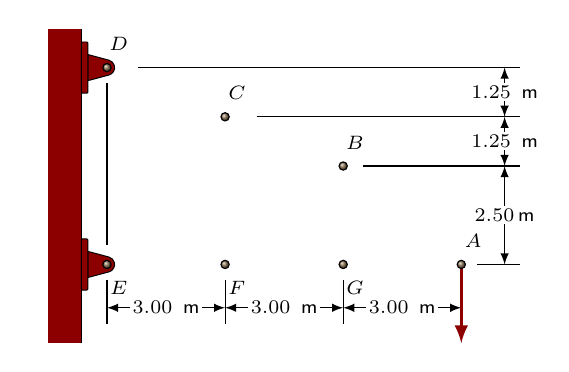
\begin{tikzpicture}



	\def\offset{0.2}
	
	\coordinate (E) at (0,0);
	\coordinate (F) at (1.5,0);
	\coordinate (G) at (3,0);
	\coordinate (A) at (4.5,0);
	\coordinate (B) at (3,1.25);
	\coordinate (C) at (1.5,1.875);
	\coordinate (D) at (0,2.5);
	\coordinate (Right) at ($ (A)+(0.75,0)$);
	\coordinate (Bottom) at ($ (A)+(0,-0.75)$);

	\fill[statsMaroon] ($(D)+(-0.325,0.5)$) rectangle ($(E)+(-.75,-1)$);
	\draw ($(D)+(-0.325,0.5)$) -- ($(E)+(-0.325,-1)$);


	\gettikzxy{(A)}{\ax}{\ay}
	\gettikzxy{(B)}{\bx}{\by}
	\gettikzxy{(C)}{\cx}{\cy}
	\gettikzxy{(D)}{\ddx}{\ddy}
	\gettikzxy{(E)}{\ex}{\ey}
	\gettikzxy{(F)}{\fx}{\fy}
	\gettikzxy{(G)}{\gx}{\gy}
	\gettikzxy{(Right)}{\rx}{\ry}
	\gettikzxy{(Bottom)}{\bbx}{\bby}

	\draw ($ (A)+(\offset,0)$) -- (\rx,\ay);
	\draw ($ (B)+(1.25*\offset,0)$) -- (\rx,\by);
	\draw ($ (C)+(2*\offset,0)$) -- (\rx,\cy);
	\draw ($ (D)+(2*\offset,0)$) -- (\rx,\ddy);
	\draw ($ (D)+(0, -\offset)$) -- (\ex,\ey+1.25*\offset cm);
	\draw ($ (E)+(0, -\offset)$) -- (\ex,\bby);
	\draw ($ (F)+(0, -\offset)$) -- (\fx,\bby);
	\draw ($ (G)+(0, -\offset)$) -- (\gx,\bby);
	\draw ($ (A)+(0, -\offset)$) -- (\ax,\bby);

	\small
	\draw[latex-latex] (\ex,\bby+\offset cm) -- node[fill=white, inner sep=0.35mm] {\scriptsize $3.00\,$ m}(\fx,\bby+\offset cm);
	\draw[latex-latex] (\fx,\bby+\offset cm) -- node[fill=white, inner sep=0.35mm] {\scriptsize $3.00\,$ m}(\gx,\bby+\offset cm);
	\draw[latex-latex] (\gx,\bby+\offset cm) -- node[fill=white, inner sep=0.35mm] {\scriptsize $3.00\,$ m}(\ax,\bby+\offset cm);
	\draw[latex-latex] (\rx-\offset cm,\ay) -- node[fill=white, inner sep=0.35mm] {\scriptsize $2.50\,\mathsf{ m}$}(\rx-\offset cm,\by);
	\draw[latex-latex] (\rx-\offset cm,\by) -- node[fill=white, inner sep=0.35mm] {\scriptsize $1.25\,$ m}(\rx-\offset cm,\cy);
	\draw[latex-latex] (\rx-\offset cm,\cy) -- node[fill=white, inner sep=0.35mm] {\scriptsize $1.25\,$ m}(\rx-\offset cm,\ddy);
	\normalsize

	% \pgfoonew \BC=new rr(B,C,Burlywood1,black, 0.2)
	% \pgfoonew \CD=new rr(C,D,Burlywood1,black, 0.2)
	% \pgfoonew \EF=new rr(E,F,Burlywood1,black, 0.2)
	% \pgfoonew \FG=new rr(G,F,Burlywood1,black, 0.2)
	% \pgfoonew \AG=new rr(A,G,Burlywood1,black, 0.2)
	% \pgfoonew \AB=new rr(A,B,Burlywood1,black, 0.2)
	% \pgfoonew \CE=new rr(C,E,Burlywood1,black, 0.2)
	% \pgfoonew \BF=new rr(B,F,Burlywood1,black, 0.2)
	% \pgfoonew \CF=new rr(C,F,Burlywood1,black, 0.2)
	% \pgfoonew \BG=new rr(B,G,Burlywood1,black, 0.2)

	 
	 \Member{B}{C}{Cornsilk4}{white}{black}{0.2}{1.125}{0.25}
	 \Member{C}{D}{Cornsilk4}{white}{black}{0.2}{1.125}{0.25}
	 \Member{A}{G}{Cornsilk4}{white}{black}{0.2}{1.125}{0.25}
	 \Member{A}{B}{Cornsilk4}{white}{black}{0.2}{1.125}{0.25}
	 \Member{F}{G}{Cornsilk4}{white}{black}{0.2}{1.125}{0.25}
	 \Member{F}{E}{Cornsilk4}{white}{black}{0.2}{1.125}{0.25}
	 \Member{B}{F}{Cornsilk4}{white}{black}{0.2}{1.125}{0.25}
	 \Member{B}{G}{Cornsilk4}{white}{black}{0.2}{1.125}{0.25}
	 \Member{C}{E}{Cornsilk4}{white}{black}{0.2}{1.125}{0.25}
	 \Member{C}{F}{Cornsilk4}{white}{black}{0.2}{1.125}{0.25}

	\PC[-90]{D}{statsMaroon}{black}{0.325}{0.125}
	\PC[-90]{E}{statsMaroon}{black}{0.325}{0.125}

	\draw[very thick, statsMaroon, -latex] (A) -- +(0,-1);

	\shadedraw[ball color=Burlywood4] (A) circle (1.5pt) node[xshift=1.5mm, yshift=3mm] {\scriptsize $A$};
	\shadedraw[ball color=Burlywood4] (B) circle (1.5pt) node[xshift=1.5mm, yshift=3mm] {\scriptsize $B$};
	\shadedraw[ball color=Burlywood4] (C) circle (1.5pt) node[xshift=1.5mm, yshift=3mm] {\scriptsize $C$};
	\shadedraw[ball color=Burlywood4] (D) circle (1.5pt) node[xshift=1.5mm, yshift=3mm] {\scriptsize $D$};
	\shadedraw[ball color=Burlywood4] (E) circle (1.5pt) node[xshift=1.5mm, yshift=-3mm] {\scriptsize $E$};
	\shadedraw[ball color=Burlywood4] (F) circle (1.5pt) node[xshift=1.5mm, yshift=-3mm] {\scriptsize $F$};
	\shadedraw[ball color=Burlywood4] (G) circle (1.5pt) node[xshift=1.5mm, yshift=-3mm] {\scriptsize $G$};
\pgfresetboundingbox
\draw[white] ($ (D)+ (-1,0.5) $) rectangle ($ (A)+(1,-1) $);

\end{tikzpicture}

	}
\end{textblock*}

\begin{textblock*}{3in}(1in, 1in)
	\cbox{
		1) Use the Pythagorean Theorem to determine the lengths of $CE$ and $CB$
	}
\end{textblock*}

\begin{textblock*}{6.875in}(1in, 5in)
	\cbox{
		2) Use the tangent function to calculate $\angle CEF$
	}
\end{textblock*}

\begin{textblock*}{6.875in}(1in, 7in)
	\cbox{
		3) Use $\angle CEF$ just found and the sine rule to verify the length of $CE$ found in 1) above.
	}
\end{textblock*}

\begin{textblock*}{6.875in}(1in, 9in)
	\cbox{
		4) Use the cosine function and the length of $CB$ found earlier to calculate the angle between $BC$ and the horizontal.
	}
\end{textblock*}

.\newpage

%%%%%%%%%%%%%%%%%%%%%%%%%%%%%%%%%%%%%%%%%%%%%%%%%%%%%%%%%%%%%%%%%%%%%%%%%%%%%%%%%%%%%%%%%%%%%%%%%%%%%%%%%%%

\begin{textblock*}{1.0\textwidth}(1in, 0.25in)
	\begin{tikzpicture}[line width= 0.3mm, scale=1.0525]
		\draw[ color=gridLight, step=0.25in] (0,0) grid (7in,10in);
	\end{tikzpicture}
\end{textblock*}

\begin{textblock*}{6.75in}(1in, 0.125in)
	\cbox{
		5) Use the tangent function to verify the previous result.
	}
\end{textblock*}

\def\scale{0.7}
\normalsize

\begin{textblock*}{2.25in}(5.6in, 1.75in)
	\cbox{
		\centering
		% !TEX root = ../../Beamer/statikz/statikz.tex


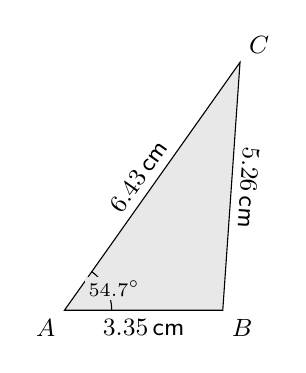
\begin{tikzpicture}[scale=0.6]

	\coordinate (A) at (0,0);
	\coordinate (B) at ($ (A)+(3.35, 0)$);
	\coordinate (C) at ($ (A)+(54.7:6.43)$);
	
  

	\small
	\filldraw[fill=Gainsboro!65, draw=black] (A) -- (B) --  (C) --  cycle;
  
	\path (A) -- (C) node[midway, sloped, above] {$6.43\,$cm};
	\path (C) -- (B) node[midway, sloped, above, rotate=180] {$5.26\,$cm};
	\path (A) -- (B) node[midway, sloped, below] {$3.35\,$cm};
	\draw[below right] (B) node {$B$};
	\draw[below left] (A) node {$A$};
	\draw[above right] (C) node {$C$};

	\draw ($ (A)+(54.7:1) $) arc (54.7:0:1)node[midway, fill=Gainsboro!65, inner sep=0.5mm,xshift=1mm] {\scriptsize $ 54.7\deg $};
  

	% \node[xshift=-0.5cm, yshift=0.15cm] at (C) {$\theta $};



\end{tikzpicture}

	}
\end{textblock*}

\begin{textblock*}{3in}(1in, 1.75in)
	\cbox{
		6) Using the sine rule, find $\angle ACB$.
	}
\end{textblock*}

\begin{textblock*}{6.875in}(1in, 4.5in)
	\cbox{
		7) Using the sine rule, find $\angle ABC$.
	}
\end{textblock*}

\begin{textblock*}{6.875in}(1in, 6.5in)
	\cbox{
		8) Sum the interior angles of the triangle.
	}
\end{textblock*}

\begin{textblock*}{2.25in}(5.6in, 8in)
	\cbox{
		\centering
		% !TEX root = ../../Presentations/01MathReview/01STCS200MathReview.tex

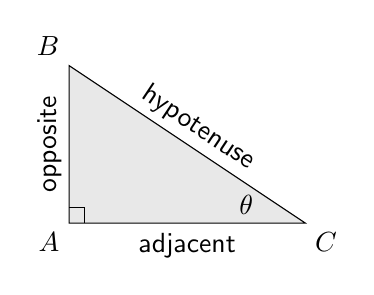
\begin{tikzpicture}

	\coordinate (A) at (0,0);
	\coordinate (B) at (0,2);
	\coordinate (C) at (3,0);

	\filldraw[fill=Gainsboro!65, draw=black] (A) -- (B) -- (C) -- cycle;
	\draw ($ (A)+(0.2,0) $) -- ++(0,0.2) -- ++(-0.2,0);

	\draw[above left] (B) node {$B$};
	\draw[below left] (A) node {$A$};
	\draw[below right] (C) node {$C$};

	
		\path (B) -- (C) node[midway, sloped, yshift=0.25cm] {hypotenuse};
		\path (A) -- (B) node[midway, sloped, yshift=0.25cm] {opposite};
		\node[below] at ($ (A)!0.5!(C) $) {adjacent};
		\node at ($ (C)+(-0.75,0.225) $) {$\theta$};


\end{tikzpicture}
	}
\end{textblock*}

\begin{textblock*}{4in}(1in, 8in)
	\cbox{
		9) Using the cosine rule, determine $\angle ABC$ \lb\lb
		10) Compare the value for $\angle ABC$ with the value calculated earlier.
	}
\end{textblock*}

.\newpage

%%%%%%%%%%%%%%%%%%%%%%%%%%%%%%%%%%%%%%%%%%%%%%%%%%%%%%%%%%%%%%%%%%%%%%%%%%%%%%%%%%%%%%%%%%%%%%%%%%%%%%%%%%%

\begin{textblock*}{1.0\textwidth}(1in, 0.125in)
	\begin{tikzpicture}[line width= 0.3mm, scale=1.0525]
		\draw[ color=gridLight, step=0.25in] (0,0) grid (7in,10in);
	\end{tikzpicture}
\end{textblock*}

\begin{textblock*}{2.75in}(5.1in, 0in)
	\cbox{
		\centering
		\fig[0.35]{../../Figs/01MathReview/simTriangles}
	}
\end{textblock*}

\begin{textblock*}{3.525in}(1in, 0in)
	\cbox{
		$ABCD$ is a rigid (i.e., it does not deform) plate, pinned at $C$. \parm
		When horizontal force $P$ is applied at $A$, $ABCD$ rotates about $C$ and $A$ deflects 2.45~mm horizontally rightwards. \parm
		Assume that $BF$ remains horizontal and that $DE$ remains vertical.\parm
		11) Determine $\delta_{BF}$, the change in length of $BF$. \parm
		12) Determine $\delta_{DE}$, the change in length of $DE$.
	}
\end{textblock*}

\begin{textblock*}{1.75in}(6.1in, 6in)
	\cbox{
		\centering
		\fig[0.35]{../../Figs/01MathReview/simTrianglesC}
	}
\end{textblock*}

\begin{textblock*}{4.5in}(1in, 6in)
	\cbox{
		13) Show that right triangles $\triangle ABC$, $\triangle ABD$ and $\triangle ACD$ all have the same angles (i.e. they are all similar).
	}
\end{textblock*}

\begin{textblock*}{6.875in}(1in, 9in)
	\cbox{
		14) Given that $AC=100\text{ mm}$ and $AD=65\text{ mm}$, determine $\angle ACD$ and $\angle ABD$.
	}
\end{textblock*}

%%%%%%%%%%%%%%%%%%%%%%%%%%%%%%%%%%%%%%%%%%%%%%%%%%%%%%%%%%%%%%%%

.\newpage

\begin{textblock*}{1.0\textwidth}(1in, 0.125in)
	\begin{tikzpicture}[line width= 0.3mm, scale=1.0525]
		\draw[ color=gridLight, step=0.25in] (0,0) grid (7in,10in);
	\end{tikzpicture}
\end{textblock*}

\begin{textblock*}{6.875in}(1in, 0in)
	\cbox{
		15) Find the remaining lengths: $AB$, $BD$ and $CD$.
	}
\end{textblock*}

\begin{textblock*}{6.875in}(1in, 3in)
	\cbox{
		16) Verify the lengths found above by using the Pythagorean Theorem on $\triangle ABC$
	}
\end{textblock*}

\begin{textblock*}{2.75in}(5.1in, 4.5in)
	\cbox{
		\centering
		\fig[0.75]{../../Figs/01MathReview/conc1}
	}
\end{textblock*}

\begin{textblock*}{3.5in}(1in, 4.5in)
	\cbox{
		17) Find $\theta_{AC}$.\qquad\qquad\qquad\qquad
		18) Find $\theta_{BC}$.
	}
\end{textblock*}


.\newpage

%%%%%%%%%%%%%%%%%%%%%%%%%%%%%%%%%%%%%%%%%%%%%%%%%%%%%%%%%%%%%%%%%%%%%%%%%%%%%%%%%%%%%%%%%%%%%%%%%%%%%%%%%%%

\begin{textblock*}{1.0\textwidth}(1in, 0.125in)
	\begin{tikzpicture}[line width= 0.3mm, scale=1.0525]
		\draw[ color=gridLight, step=0.25in] (0,0) grid (7in,10in);
	\end{tikzpicture}
\end{textblock*}

\begin{textblock*}{2in}(1in, 2.5in)
	\cbox{
		19) Solve $a^2=b^2+c^2$ for $b$.
	}
\end{textblock*}

\begin{textblock*}{2in}(1in, 4.5in)
	\cbox{
		20) Solve $V=\frac43 \pi r^3$ for $r$.
	}
\end{textblock*}

\begin{textblock*}{3in}(1in, 6.5in)
	\cbox{
		21) Solve $c^2=a^2+b^2-2bc\cos C$ for $\cos C$.
	}
\end{textblock*}

\begin{textblock*}{3in}(1in, 8.5in)
	\cbox{
		22) Solve $b^2=a^2+c^2-2ac\cos B$ for $B$.
	}
\end{textblock*}

.\newpage

%%%%%%%%%%%%%%%%%%%%%%%%%%%%%%%%%%%%%%%%%%%%%%%%%%%%%%%%%%%%%%%%

\begin{textblock*}{1.0\textwidth}(1in, 0.125in)
	\begin{tikzpicture}[line width= 0.3mm, scale=1.0525]
		\draw[ color=gridLight, step=0.25in] (0,0) grid (7in,10in);
	\end{tikzpicture}
\end{textblock*}

\begin{textblock*}{6.875in}(1in, 0in)
	\cbox{
		$$  Q=\frac{CD^{2.63}\left(\frac{h_L}{L}\right)^{0.54}}{279000}$$\parb
		23)  Solve the equation for $h_L$, then evaluate $h_L$ using the values $Q=135$, $C=120$, $D=202.7$ and $L=1200$
	}
\end{textblock*}

\begin{textblock*}{6.875in}(1in, 4in)
	\cbox{
		 \begin{align*}
			 0.36911x + 0.61633y & = 2011.1 \\
	 			0.78748y - 0.92938x & = 0
	\end{align*}\parm
	24) and 25) Find the values of $x$ and  $y$
	}
\end{textblock*}

.\newpage
%%%%%%%%%%%%%%%%%%%%%%%%%%%%%%%%%%%%%%%%%%%%%%%%%%%%%%%%%%%%%%%%
%%%%%%%%%%%%%%%%%%%%%%%%%%%%%%%%%%%%%%%%%%%%%%%%%%%%%%%%%%%%%%%%

\begin{textblock*}{1.0\textwidth}(1in, 0.125in)
	\begin{tikzpicture}[line width= 0.3mm, scale=1.0525]
		\draw[ color=gridLight, step=0.25in] (0,0) grid (7in,10in);
	\end{tikzpicture}
\end{textblock*}

\begin{textblock*}{6.875in}(1in, 0in)
	\cbox{

	\begin{align*}
		\setcounter{equation}{0}
		F_{BC}\sin15^\circ + F_{AC}\cos35^\circ + 1030.1 & = 0 \\
		F_{BC}\cos 15^\circ+F_{AC}\sin35^\circ           & = 0
	\end{align*}

	\parm
	26) and 27) Determine $F_{AC}$ and $F_{BC}$
	}
\end{textblock*}


\end{document}
